\documentclass[class=report, crop=false, 12pt,a4paper]{standalone}
\usepackage{enumitem}
\usepackage{multicol}
\usepackage{etoolbox}
\AtBeginEnvironment{quote}{\singlespacing\small}
\usepackage{setspace}
\onehalfspacing
\usepackage{graphicx}
\usepackage{float}
\usepackage{amsmath}
\usepackage{amssymb}
\usepackage{siunitx}
\sisetup{detect-all}
\begin{document}
\section{Coordinate systems and velocity fields}
Fluid flow can be classified in four ways:
\begin{enumerate}[noitemsep]
  \item Viscous/inviscid - when the viscosity of a fluid is equal to zero e.g. viscous -  blood flow through a capillary, honey and inviscid - tornado, stirring tea.
  \item Laminar and turbulent flow - Reynold's number. This is a measure used to determine whether a flow is likely to be laminar or turbulent.
  \item Compressible or incompressible - density is constant/does not change with time e.g. compressible - clouds, gas turbines and incompressible - oil pipelines, water dams.
  \item Steady and unsteady flow - the velocity at a particular point in space does not change with time and eddy formations or the opposite with eddies and turbulence.
\end{enumerate}
\subsection{Coordinate systems and labelling}
There are various notations used.
\subsubsection{Cartesian coordinates}
Position: x, y, z
\begin{equation} 
  \underline{x} = 
  \begin{pmatrix}
    x\\
    y\\
    z
  \end{pmatrix} = 
  x\underline{i} + y\underline{j} + z\underline{k} 
\end{equation}
Velocity: u, v, w
\begin{equation} 
  \underline{v} = 
  \begin{pmatrix}
    u\\
    v\\
    w
  \end{pmatrix} = 
  u\underline{i} + v\underline{j} + w\underline{k} 
\end{equation}
\subsubsection{Forces}
Forces can either be applied to the body or on one of its surfaces.
\begin{itemize}[noitemsep]
  \item Body forces - The force acts at the centre of each increment of mass e.g. gravity.
  \item Surface flows - The force acts at the surface of each increment of mass e.g. shear stress.
\end{itemize}
As there are two types of forces, we need a consistent labelling system to distinguish them. 
\begin{figure}[H]
  \centering
  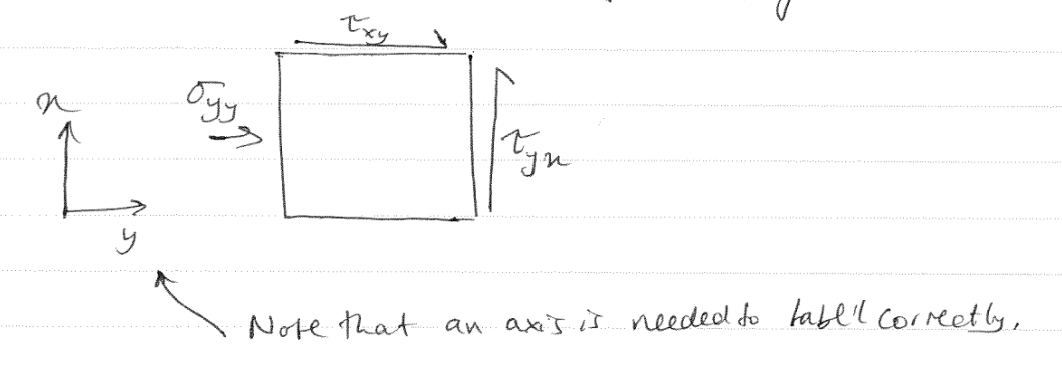
\includegraphics[width = \textwidth]{../img/ForceDiagramFluids}
  \caption{Force Diagram on an increment of fluid}
\end{figure}
\( \sigma_yy \) The first subscript refers to the face that the force is applied to. The second subscript is the direction the force acts in.
\subsubsection{Incremental element of volume}
Consider an incremental volume with dimensions: dx, dy, dz.
\begin{figure}[H]
  \centering
  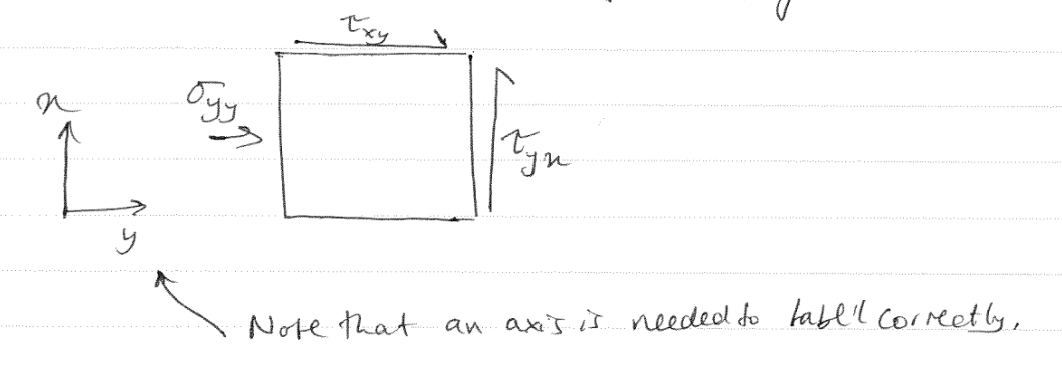
\includegraphics[width = \textwidth]{../img/ForceDiagramFluids}
  \caption{Force Diagram on an increment of fluid}
\end{figure}
There is a variation of fluid speeds in this box. Each component of the velocity can vary in each of these directions. The x-component of velocity, n, could vary with x, y or z independently.
\begin{equation} 
  \frac{\partial n}{\partial x}, \ \frac{\partial n}{\partial y}, \ \frac{\partial n}{\partial z} 
\end{equation}
and the same goes to v and w.
\subsection{Velocity Fields}
A field is a three dimensional description of a field parameter in space. For example:
\begin{equation}  
  \underline{v} = u
  \begin{pmatrix}
    x\\
    y\\
    z
  \end{pmatrix} \underline{i} + v
  \begin{pmatrix}
    x\\
    y\\
    z
  \end{pmatrix} \underline{j} + w
  \begin{pmatrix}
    x\\
    y\\
    z
  \end{pmatrix} \underline{k}
\end{equation}
More generally, the flow field can be a function of time, t (this is unsteady flow.)
\begin{equation}
  \underline{v} = u
  \begin{pmatrix}
    x\\
    y\\
    z\\
    t
  \end{pmatrix} \underline{i} + v
  \begin{pmatrix}
    x\\
    y\\
    z\\
    t
  \end{pmatrix} \underline{j} + w
  \begin{pmatrix}
    x\\
    y\\
    z\\
    t
  \end{pmatrix} \underline{k}
\end{equation}
You can also get acceleration fields. Velocity and acceleration fields are vector fields as it has magnitude and direction. A scalar field only has magnitude e.g. Pressure, temperature and density fields.
\subsection{Eularian and Lagrangian flow descriptions}
There are two general approaches in analysing fluid mechanics problems:
\begin{enumerate}[noitemsep]
  \item Eularian method - this uses fields to describe the flow at a specific position in time and space. 
  \item Lagrangian method - this describes what happens to an individual particle with time g.g ocean drifters, measuring conditions as they float freely through the oceans.
\end{enumerate}
\subsection{One-, two- and three- dimensional flows}
Most flows are 3D flows, However, if one of the velocity components may be small (in some sense) relative to the other components then it may be reasonable to neglect the smaller components and assume 2D flow. That is \( \underline{v} = u\underline{i} + v\underline{j} \). Sometimes two of the components may be negligible so it can be approximated to one dimensional flow. That is \( \underline{v} = u\underline{i} \).

For many flows, one dimensional flow will provide a reasonable approximation, whereas in others would produce erroneous results.
\begin{gather} 
  \textrm{Steady flow} \rightarrow \frac{\partial v}{\partial t} = 0\\
  \textrm{Unsteady flow} \rightarrow \frac{\partial v}{\partial t} \neq 0 
\end{gather}
\subsection{Streamlines, streaklines and pathlines}
\begin{itemize}[noitemsep]
  \item Pathlines - the line traced out by a given particle as it flows from one point to another.
  \item Streaklines - A line that is created by particles in a flow that have previously passed through a common point.
  \item Streamlines - A line that is tangent to the velocity to the velocity field (if flow is steady).
\end{itemize}
If the flow is steady nothing at a fixed point changes with time, so the streamlines are fixed in space. If unsteady, the streamlines will change with time. Streamlines are obtained by integration. 
\begin{equation} 
  \frac{dy}{dx} = \frac{v}{u} 
\end{equation}
v and u are usually functions of x and y and so integration after separating variables can be done and graphs drawn for various constant of integration. If steady, streamline = streakline.
\subsection{The acceleration field}
To apply Newton's second law, we need the acceleration. For the Lagrangian method, \( a = a(t) \) for each particle. For the Eularian description, we can find the acceleration field, which provides the acceleration of given points in a field. We will discuss how to get this if the velocity field is known. 
\subsection{The material derivatives}
Consider a fluid particle moving along its pathline. In general, the particles velocity, denoted \(V_A\) for particle A, is a function of location and time. That is
\begin{equation} 
  V_A = V_A(V_A, \ b) = V_A \left[ x_A(t), \ y_A(t), \ z_A(t), t \right] = V_A \left[ x_A, \ y_A, \ z_A,\  t \right] 
\end{equation}
By definition, acceleration is the rate of change of velocity. We have to apply the chain rule as acceleration may change due to a change in position or time. 
\begin{gather} 
  \underline{a}_A(t) = \frac{dV_A}{dt} = \frac{\partial V_A}{\partial t} \frac{dt}{dt} + \frac{\partial V_A}{\partial x} \frac{dx_A}{dt} + \frac{\partial V_A}{\partial y} \frac{dy_A}{dt} + \frac{\partial V_A}{\partial z} \frac{dz_A}{dt} \\
  = \frac{\partial V_A}{\partial t} + \frac{\partial V_A}{\partial x} \frac{dx_A}{dt} + \frac{\partial V_A}{\partial y} \frac{dy_A}{dt} + \frac{\partial V_A}{\partial z} \frac{dz_A}{dt} \\
  \textrm{since } u_A = \frac{dx_A}{dt}, \ v_A = \frac{dy_A}{dt}, \ w_A = \frac{dz_A}{dt} \\
  \underline{a}_A = \frac{\partial V_A}{\partial t} + \frac{\partial V_A}{\partial x} u_A + \frac{\partial V_A}{\partial y} v_A + \frac{\partial V_A}{\partial z} w_A
\end{gather}
This applies for any project and so we can drop the subscript.
\begin{equation} 
  \underline{a} = \frac{\partial V}{\partial t} + \frac{\partial V}{\partial x} u + \frac{\partial V}{\partial y} v + \frac{\partial V}{\partial z} w 
\end{equation}
This is a vector result where scalar components can be written as:
\begin{gather}
  a_x = \frac{\partial u}{\partial t} + u\frac{\partial u}{\partial x} + v\frac{\partial u}{\partial y} + w\frac{\partial u}{\partial z} \\
  a_y = \frac{\partial v}{\partial t} + u\frac{\partial u}{\partial x} + v\frac{\partial u}{\partial y} + w\frac{\partial u}{\partial z} \\
  a_z = \frac{\partial w}{\partial t} + u\frac{\partial u}{\partial x} + v\frac{\partial u}{\partial y} + w\frac{\partial u}{\partial z}
\end{gather}
All of this is written in shorthand as:
\begin{equation} 
  \underline{a} = \frac{Dv}{Dt}
\end{equation}
Where the operator \( \frac{D}{Dt}\) is the material derivative. 
\begin{equation} 
  \frac{D}{Dt}() = \left[\frac{\partial ()}{\partial t} \right] \textrm{(A)} + \left[u\frac{\partial ()}{\partial x} + v\frac{\partial ()}{\partial y} + w\frac{\partial ()}{\partial z} \right] \textrm{(B)}
\end{equation}
Where A is the local derivative and B is the convective derivative. 

If the parameter involved is acceleration, term (A) is called \emph{local acceleration} for steady flow this is equal to zero. \( \frac{\partial v}{\partial t} = 0 \). This physically means there is no change in flow parameter at a fixed point in space if the flow is steady. 

The collection of terms labelled (B) are called the convective derivative. It represents the fact that a flow property associated with a fluid particle may vary because of the motion of the particle from one place to another. This contribution occurs when the parameter of concern is acceleration, then section (B) is called the convective acceleration. 
\subsection{Streamline coordinates}
in the streamline C.S. the flow is described in terms of one coordinate along the streamlines, denoted s, and the second coordinate normal to the streamlines, denoted n. Unit vectors in this direction are denoted by \( \underline{\hat{s}} \) and \( \underline{\hat{n}} \). The flow plane is covered by an orthogonal curved net of coordinate lines. s and n are always perpendicular, but the lines of constant s or constant n are not necessarily straight. Note that velocity is always tangent to the s direction. Thus:
\begin{equation} 
  \underline{v} = v\underline{\hat{s}}
\end{equation}
For steady, 2D flow, the acceleration is:
\begin{equation} 
  \underline{a} = \frac{Dv}{Dt} = a_s \hat{s} + a_n \hat{n}
\end{equation}
Where \( a_s \hat{s} \) is the acceleration in the streamline direction and \( a_n \hat{n} \) is the acceleration in the normal direction. 

In general, for steady flow, both the speed and the flow direction are a function of location.
\begin{equation} 
  v = v(s, n) \textrm{ and } \underline{\hat{s}} = \underline{\hat{s}}(s, n)
\end{equation}
For a given particle, the value \(dt \) s changes with time but the value of n remains fixed as the particle flows along a streamline defined by n = constant. (note: pathlines = streamlines during steady flow). Thus: 
\begin{equation} 
  \underline{a} = \frac{Dv}{Dt} = \frac{D}{Dt}(v\hat{s}) = \frac{Dv}{Dt}\underline{\hat{s}} + v \frac{D\underline{\hat{s}}}{Dt}
\end{equation}
Applying the material derivative,
\begin{equation}
  \underline{a} = \left( \frac{\partial v}{\partial t} + \frac{\partial v}{\partial s}\frac{ds}{dt} + \frac{\partial v}{\partial n}\frac{dn}{dt} \right) \hat{s} + v \left( \frac{\partial \underline{\hat{s}}}{\partial t} + \frac{\partial \underline{\hat{s}}}{\partial s}\frac{ds}{dt} + \frac{\partial \underline{\hat{s}}}{\partial n}\frac{dn}{dt} \right)
\end{equation}
For steady flow, this simplifies too:
\begin{equation} 
  \underline{a} = \left( v\frac{\partial v}{\partial s} \right) \underline{\hat{s}} + v \left( v\frac{\partial \underline{\hat{s}}}{\partial s} \right)
\end{equation}
This equation can also be rewritten as:
\begin{equation} 
  \underline{a} = v\frac{\partial v}{\partial s} \underline{\hat{s}} + \frac{v^2}{R} \underline{\hat{n}}
\end{equation}
Or,
\begin{align} 
  a_s &= v\frac{\partial v}{\partial s}\\
  a_n &= \frac{v^2}{R} 
\end{align}
Where \(a_s\) is the streamwise/acceleration convective and \(a_n\) is the normal/acceleration centrifugal.
\subsection{Example question}
Given a velocity field:
\begin{equation}
  \vec{V} = Ax\hat{i} - Ay\hat{j}
\end{equation}
where x and y are in metres, $A = 0.3 \ \si{\per\second}$, find:
\begin{enumerate}[noitemsep]
  \item Equation of the streamlines in the xy plane.
  \item Streamline plot through point (2, 8).
  \item Velocity of particle at point (2, 8).
  \item Position at $t = 6 \ \si{\second}$ of particle located at (2, 8) $t =0$.
\end{enumerate}
\subsubsection{1}
Streamlines are lines drawn in the flow field such that at a given instant they are tangent to the direction of flow at every point. Consequently,
\begin{equation}
  \left( \frac{dy}{dx} \right)_{streamline} = \frac{v}{u} = \frac{-Ay}{Ax} = \frac{-y}{x}
\end{equation}
Separating variables and integrating, we obtain,
\begin{equation}
  \int \frac{dy}{y} = - \int \frac{dx}{x}
\end{equation}
Or
\begin{equation}
  \ln{y} = - \ln{x} + c_1
\end{equation}
This can be written as
\begin{equation}
  xy = c
\end{equation}
\subsubsection{2}
For the streamline passing through the point $(x_0, \ y_0) = (2, \ 8)$ the constant, c, has a value of 16 and the equation of the streamline through the point (2, 8) is
\begin{equation}
  xy = x_0y_0 = 16 \ \si{\meter\squared}
\end{equation}
This is sketched below.
\begin{figure}[h]
  \centering
  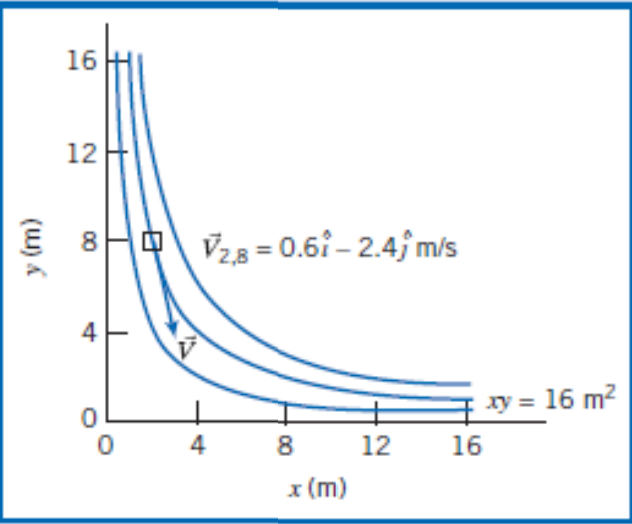
\includegraphics[width = 0.5\textwidth]{../img/streamlineexampleqgraph}
  \caption{Plot to show streamlines}
\end{figure}
\subsubsection{3}
The velocity field is $\vec{V} = Ax\hat{i} - Ay\hat{j}$. At the point (2, 8), the velocity is,
\begin{equation}
  \vec{V} = A(x\hat{i} - y\hat{j}) = 0.3(2\hat{i} - 8 \hat{j}) = 0.6\hat{i} - 2.4\hat{j} \ \si{\meter\per\second}
\end{equation}
\subsubsection{4}
A particle moving in the flow field will have velocity given by
\begin{equation}
  \vec{V} = A(x\hat{i} - y\hat{j})
\end{equation}
Thus
\begin{equation}
  u_p = \frac{dx}{dt} = Ax \textrm{ and } u_p = \frac{dy}{dt} = -Ay
\end{equation}
Separating the variables and integrating (in each equation) gives
\begin{equation}
  \int_{x_0}^{x_1} \frac{dx}{x} = \int_0^t A dt \textrm{ and } \int_{y_0}^{y_1} \frac{dy}{y} = \int_0^t -A dt
\end{equation}
Then
\begin{equation}
  \ln{\frac{x}{x_0}} = At \textrm{ and } \ln{\frac{y}{y_0}} = -At
\end{equation}
or 
\begin{equation}
  x = x_0 e^{At} \textrm{ and } y = y_0 e^{-At}
\end{equation}
At $t=6$
\begin{equation}
  x = 12.1 \ \si{\meter} \textrm{ and } y = 1.32 \ \si{\meter}
\end{equation}
At $t=6$, particle is at (12.1, 1.32) \si{\meter}
\end{document}